\chapter{Literature}
\section{Structures of \acs{QA} on the Ag(100) surface}

In principle, two primary structures are observed to form on the Ag(100) surface: the $\alpha$- and $\beta$-Phase. A thorough examination of these two phases has been conducted by N. Humberg.\autocite{Humberg2024}

It has been ascertained that the formation of the $\alpha$-phase occurs subsequent to the deposition of the \ac{QA} molecules onto the Ag(100) surface at a sample temperature of 300~\si{K}. This phase is composed of domains of parallel molecular chains that are flat-lying on the surface. The \ac{QA} molecules are connected via intermolecular hydrogen bonds between the keto groups of one molecular chain and the amine groups of another. It was also determined that the domains under consideration are homochiral, a finding that suggests a high degree of mobility for the \ac{QA} molecules on Ag(100) at 300~\si{K}.

In addition, the superstructure matrix of the $\alpha$-phase was determined using a \ac{SPA-LEED} image and \ac{STM} results. The following superstructure matrix was found
\begin{equation*}
\mathbf{M_\alpha} =\begin{pmatrix}
2 & 1.25 \\
-3 & 4.80 
\end{pmatrix},
\end{equation*}
which shows that the structure is of the \ac{POL} type.


The phase transition from the $\alpha$-phase to the $\beta$-phase was discovered when the sample was heated up to 500~\si{K} for 15 minutes. The phase transition is irreversible. This means that the $\alpha$-phase is metastable and is stabilized by a kinetic barrier from the intermolecular hydrogen bonds.


For the $\beta$-phase, the investigation revealed parallel molecular chains, which are comprised of dimers and manifest periodic indents. This results in a single hydrogen bond between the dimers instead of theoretical two possible hydrogen bonds. The two molecules of the dimer form two hydrogen bonds with each other. Once more, employing a \ac{SPA-LEED} image and \ac{STM} results, the superstructure matrix of the $\beta$-phase was determined as
\begin{equation*}
\mathbf{M_\beta} =\begin{pmatrix}
4 & 3 \\
-5 & 3 
\end{pmatrix},
\end{equation*}
which means that the structure is commensurate.
The structure of the $\alpha$- and $\beta$-phase corresponding to the structure model of N. Humberg is illustrated in \autoref{fig:structures_literature}.

\begin{figure}[htbp]
	\centering
	\begin{subfigure}[b]{0.49\linewidth}
		\centering
		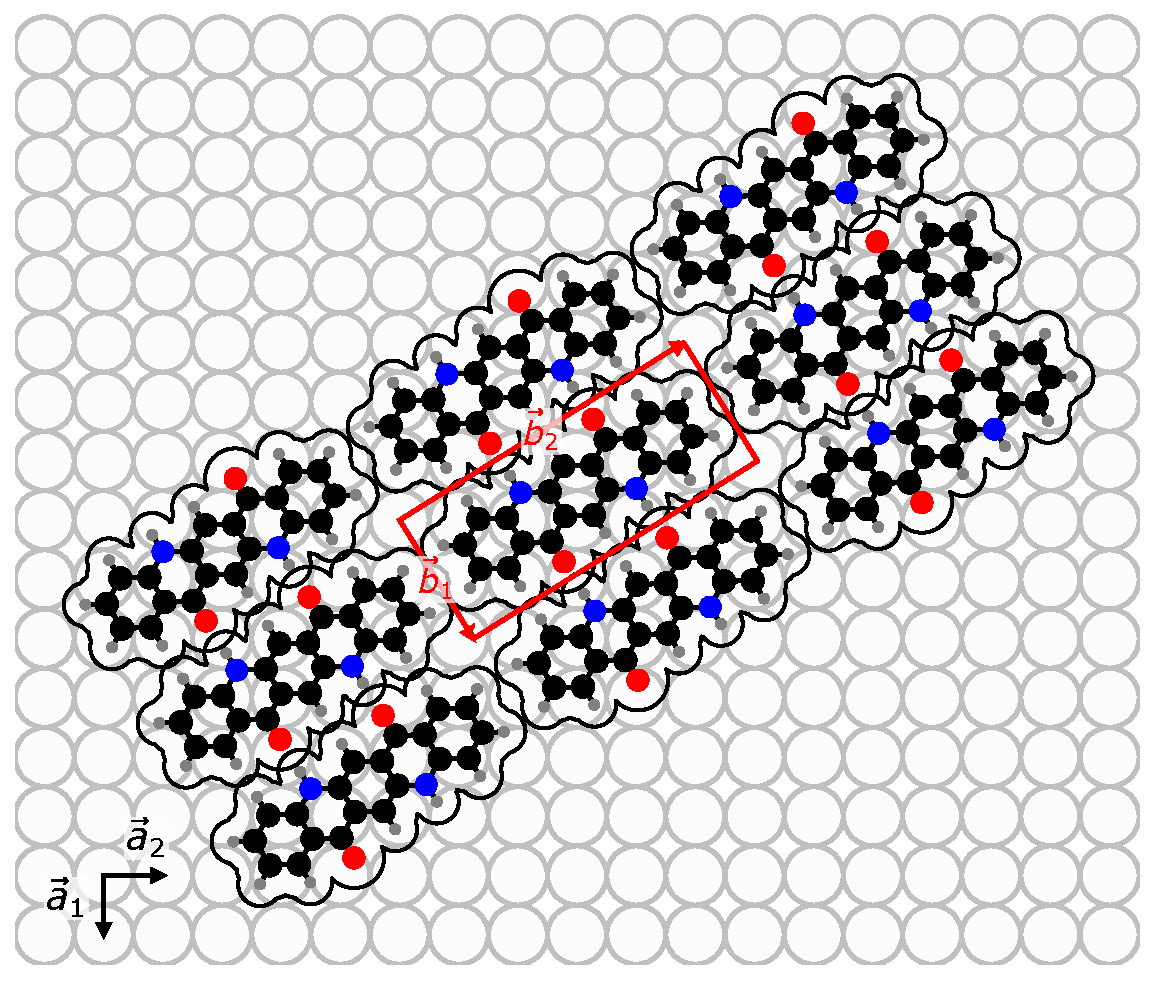
\includegraphics[width=\linewidth]{images/QA-alpha-Ag(100).pdf}
		\caption{$\alpha$-phase of \ac{QA} on Ag(100)}
	\end{subfigure}
	\hfill
	\begin{subfigure}[b]{0.49\linewidth}
		\centering
		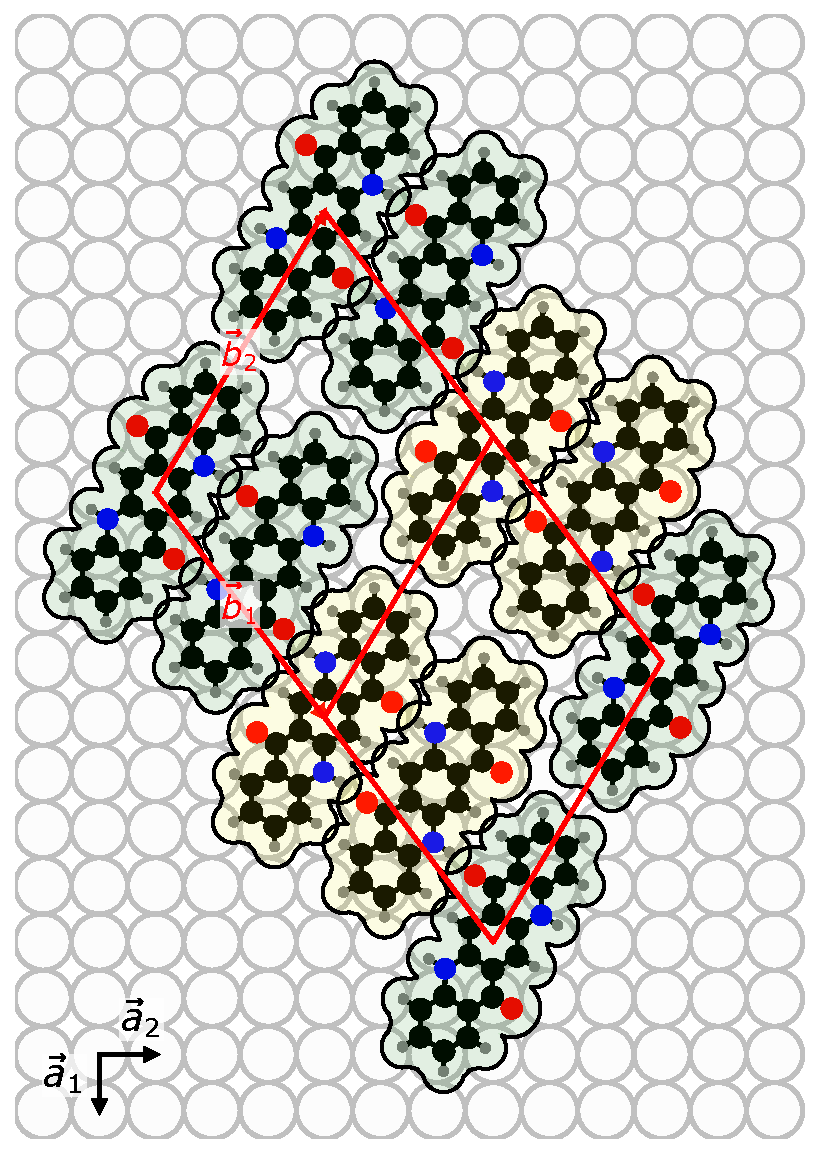
\includegraphics[width=\linewidth]{images/QA-beta-Ag(100).pdf}
		\caption{$\beta$-phase of \ac{QA} on Ag(100)}
	\end{subfigure}
	\caption{Structure models for the $\alpha$- and the $\beta$-phase of \ac{QA} on Ag(100) according to the literature \cite{Humberg2024}.}
	\label{fig:structures_literature}
\end{figure}

\cleardoublepage